\chapter*{Rilevamento della frequenza fondamentale}\label{cap:rilevamento_frequenza}

L'algoritmo utilizzato per rilevare la frequenza fondamentale è l'algoritmo \emph{Harmonic Product Spectrum}, abbreviato dall'acronimo \emph{HPS}.
Tale metodo sfrutta il fatto che quando viene suonata una nota con uno strumento musicale, l'energia del suono si concentra principalmente nella frequenza fondamentale e nelle sue armoniche, cioè i suoi multipli interi.

L'algoritmo HPS moltiplica lo spettro del segnale con un numero \emph{K-1} di versioni differenti dello spettro.
Le diverse versioni sono ottenute sotto-campionando lo spettro originale con i diversi fattori compresi tra 2 e K.
La formula \ref{formula:hps_prod} descrive la prima parte di questo algoritmo per un generico spettro X( \omega ) e un generico valore \emph{K}.

\begin{equation}\label{formula:hps_prod}
	Y(\omega) = \prod_{i=1}^K \left | X(\omega i) \right |
\end{equation}

Una volta ottenuto il prodotto, la frequenza fondamentale viene calcolata come ascissa del massimo della funzione risultante. 
La formula \ref{formula:hps_max} descrive questo secondo passaggio.

\begin{equation}\label{formula:hps_max}
	Y_{f0} = \max_{\omega_i} Y \left(\omega_i \right )
\end{equation}

 

	\begin{figure}[h]
	  \begin{center} 
	    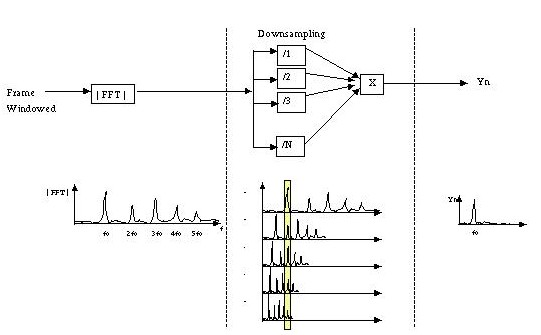
\includegraphics[width=\textwidth*\real{0.9}]{images/ch_04/processo.jpg}
	  \end{center} 
	  \caption{\textit{Rumore di registrazione}}  
	  \label{fig:rumore}
	\end{figure}


